
\subsubsection{MenuDataStructures}
Dieses Paket stellt Datenstrukturen für das Menü bereit. 
Unter anderem existiert eine Klasse MiniMapPosition, die 
die Koordinaten des Spielers auf der MiniMap speichert, 
und die Klasse SeedEntry, die zur Speicherung von Seeds 
verwendet wird. Seeds werden jedoch nicht hier gespeichert, 
sondern in einer .properties Datei die in SeedConfig
verwaltet wird.
\par

\begin{figure}[!h]
    \centering
    \centering
        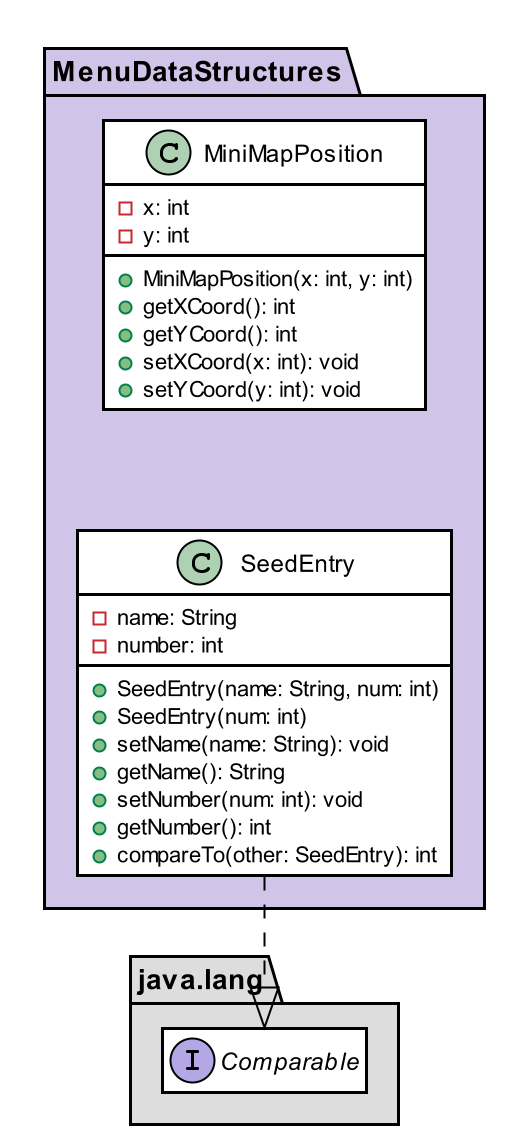
\includegraphics[width=.45\linewidth]{./GUI/GUI_Bilder/MenuDataStructures.png}
          \caption{Paket MenuDataStructures}
           \label{fig:MenuDataStructures}
\end{figure}
    \pagebreak
    \paragraph{\underline{MiniMapPosition}}\label{mmp} \mbox{}\\
        Diese Klasse stellt eine Datenstruktur für die 
        Positionen eines Spielers auf der MiniMap bereit.
        Sie besitzt eine X- und Y-Koordinate, sowie Getter
        und Setter.\\
        \par
        \textbf{Attribute}
        \begin{itemize}
            \item \textit{- int x}  
                \begin{leftbar}[0.9\linewidth]
                    Enthält die X-Koordinate eines Spielers auf 
                    der MiniMap.
                \end{leftbar}
            \item \textit{- int y} 
                \begin{leftbar}[0.9\linewidth]
                    Enthält die Y-Koordinate eines Spielers auf 
                    der MiniMap.
                \end{leftbar}
        \end{itemize}
        \textbf{Methoden}					
        \begin{itemize}
            \item \textit{+ MiniMapPosition(int x, int y)}
                \begin{leftbar}[0.9\linewidth]
                    Dieser Konstruktor speichert den übergebenen Namen und die 
                    Ziffernreihenfolge des neu erstellten Seed-Eintrag Objektes.\\
                    \textbf{@param x} Die zu setzende X-Koordinate.\\
                    \textbf{@param y} Die zu setzende Y-Koordinate.
                \end{leftbar}
            \item \textit{+ getXCoord(): int}
                \begin{leftbar}[0.9\linewidth]
                    Getter für die X-Koordinate eines Spielers auf 
                    der MiniMap.\\
                    \textbf{@return} Die X-Koordinate.
                \end{leftbar}
            \item \textit{+ getYCoord(): int}
                \begin{leftbar}[0.9\linewidth]
                    Getter für die Y-Koordinate eines Spielers auf 
                    der MiniMap.\\
                    \textbf{@return} Die Y-Koordinate.
                \end{leftbar}
            \item \textit{+ setXCoord(int x): void}
                \begin{leftbar}[0.9\linewidth]
                    Setter für die X-Koordinate eines Spielers auf 
                    der MiniMap.\\
                    \textbf{@param x} Die zu setzende X-Koordinate.
                \end{leftbar}
            \item \textit{+ setYCoord(int y): void}
                \begin{leftbar}[0.9\linewidth]
                    Setter für die Y-Koordinate eines Spielers auf 
                    der MiniMap.\\
                    \textbf{@param y} Die zu setzende Y-Koordinate.
                \end{leftbar}
        \end{itemize}

    \paragraph{\underline{SeedEntry}}\label{seedentry} \mbox{}\\
        Diese Klasse repräsentiert die Datenstruktur eines Seed Eintrages.
        Ein Seed Eintrag hat dabei immer einen Namen und eine Ziffernreihenfolge.
        Letzteres identifizert einen Seed Eintrag. Demzufolge können
        mehrere Seeds nicht die selbe Ziffernreihenfolge haben. Die Überprüfung
        findet jedoch nicht hier statt, sondern in den Menü Klassen aus dem GUI.
        Die Klasse implementiert das Comparable Interface, damit die Seed-Einträge
        später sortiert werden können.\\
        \par
        \pagebreak
        \textbf{Attribute}
        \begin{itemize}
            \item \textit{- String name}  
                \begin{leftbar}[0.9\linewidth]
                    Enthält den Namen vom Seed-Eintrag.
                \end{leftbar}
            \item \textit{- int number} 
                \begin{leftbar}[0.9\linewidth]
                    Enthält die Ziffernreihenfolge des Seed-Eintrages.
                \end{leftbar}
        \end{itemize}
        \textbf{Methoden}					
        \begin{itemize}
            \item \textit{+ SeedEntry(String name, int num)}
                \begin{leftbar}[0.9\linewidth]
                    Dieser Konstruktor speichert den übergebenen Namen und die 
                    Ziffernreihenfolge des neu erstellten Seed-Eintrag Objektes.\\
                    \textbf{@param name} Der zu setzende Name.\\
                    \textbf{@param num} Die zu setzende Ziffernreihenfolge.\\
                \end{leftbar}
            \item \textit{+ SeedEntry(int num)}
                \begin{leftbar}[0.9\linewidth]
                    Dieser Konstruktor speichert die Ziffernreihenfolge des neu 
                    erstellten Seed-Eintrag Objektes und setzt den Namen des 
                    Seed-Eintrages gleich der Ziffernreihenfolge.\\
                    \textbf{@param num} Die zu setzende Ziffernreihenfolge.\\
                \end{leftbar}
            \item \textit{+ setName(String name): void}
                \begin{leftbar}[0.9\linewidth]
                    Überschreibt den aktuellen Namen des Seed-Eintrages mit 
                    dem übergebenem String.\\
                    \textbf{@param name} Der zu speichernde Name.
                \end{leftbar}
            \item \textit{+ getName(): String}
                \begin{leftbar}[0.9\linewidth]
                    Gibt den aktuellen Namen des Seed-Eintrages zurück.\\
                    \textbf{@return} Name des Seed-Eintrages.
                \end{leftbar}
            \item \textit{+ setNumber(int num): void}
                \begin{leftbar}[0.9\linewidth]
                    Überschreibt die aktuelle Ziffernreihenfolge des Seed-Eintrages mit 
                    dem übergebenem Integer.\\
                    \textbf{@param num} Die zu speichernde Ziffernreihenfolge.\\
                \end{leftbar}
            \item \textit{+ getNumber(): int}
                \begin{leftbar}[0.9\linewidth]
                    Gibt die aktuelle Ziffernreihenfolge des Seed-Eintrages zurück.\\
                    \textbf{@return} Ziffernreihenfolge des Seed-Eintrages.
                \end{leftbar}
            \item \textit{+ compareTo(SeedEntry other): int}
                \begin{leftbar}[0.9\linewidth]
                    Siehe dazu java.lang.Comparable\#compareTo(java.lang.Object).
                \end{leftbar}
        \end{itemize}


\pagebreak